\documentclass[supercite]{HustGraduPaper}
%进行个人信息设置
\title{RIS辅助的无线通信系统的原型验证} %论文题目
\author{裴熙隆} %作者姓名
\date{\today} %日期,默认当日
\school{人工智能与自动化学院} %院系名称
\classnum{自动化1705班} %专业班级
\stunum {U201714286} %学号
\instructor{陈忠、尹海帆} %指导教师姓名

%添加自己要用的其他宏包
\usepackage{xltxtra}
\usepackage{bm}
\usepackage{array}
\usepackage{multirow}
\usepackage[caption=false,font=footnotesize]{subfig}
\usepackage{algorithm}
\usepackage{algorithmic}
\usepackage{amsthm}

\newtheorem{theorem}{\indent 定理}[section]
\newtheorem{lemma}{\indent 引理}[section]
\newtheorem{proposition}{\indent 命题}[section]
\newtheorem{corollary}{\indent 推论}[section]
\newtheorem{definition}{\indent 定义}[section]
\newtheorem{example}{\indent 例}[section]
\newtheorem{remark}{\indent 注}[section]
\renewcommand{\proofname}{\indent\bf 证明}

\begin{document}
%生成标题页 \maketitle[可选参数]\end{document}\end{document}
%可选参数:
%logo color=green/black 华中科技大学字样的颜色,绿色或者黑色,默认绿色
%line length=12em 填写信息处横线的长度,默认12em
%line font=huawenzhongsong 填写信息的字体,默认huawenzhongsong
\maketitle

%生成声明与授权书页 \statement[可选参数]
%可选参数:
%confidentiality=yes/no/true/false/empty
%是否保密,yes/true为保密;no/false为不保密,empty为不填,默认为empty
%year=5 保密年数,默认为空
\statement[confidentiality = false]

\clearpage %结束上一页
\pagenumbering{Roman} %摘要页码为大写罗马数字

%填写中文摘要内容和关键字
\begin{cnabstract}{可重构智能表面;智能反射面;无线中继;大规模多进多出系统;原型系统;现场可编程逻辑门阵列}
	%请注意使用中文分号“;”分割关键词!

	近年来,

\end{cnabstract}
%填写英文摘要内容和关键字
\begin{enabstract}{Reconfigurable intelligent surface; intelligent reflecting surface; wireless repeating; massive multiple-input multiple-output; prototype; field programmable gate array}
	%Please Use English Semicolon and a Space "; " to Separate Keys! 

	Recently,

\end{enabstract}

%生成目录 \tableofcontents[可选参数]
%可选参数:
%pagenum=yes/no/true/false 目录是否显示页码,默认为false
%toc in toc=yes/no/true/false 目录中是否有目录及其页码,默认为false
%level=4 目录级数,默认是4,即显示到subsubsubsection
%section indent=0em 目录第一级的缩进,默认是0em
%subsection indent=1.5em 目录第二级的缩进,默认是1.5em
%subsubsection indent=3.8em 目录第三级的缩进,默认是3.8em
%subsubsubsection indent=7em 目录第四级的缩进,默认是7em
%paragraph indent=11em 目录第五级的缩进,默认是11em
%subparagraph indent=13em 目录第六级的缩进,默认13em
%indent=normal/noindent/hustnoindent/sameforsubandsubsub 快速缩进设置,具体见文档
%dot sep=4.5 目录点间距,默认4.5
%section dot sep=4.5 目录第一级的点间距,默认是4.5
%subsection dot sep=4.5 目录第二级的点间距,默认是4.5
%subsubsection dot sep=4.5 目录第三级的点间距,默认是4.5
%subsubsubsection dot sep=4.5 目录第四级的点间距,默认是4.5
%paragraph dot sep=4.5 目录第五级的点间距,默认是4.5
%subparagraph dot sep=4.6 目录第六级的点间距,默认是4.5
%请注意在合适的位置放置\pagenumbering{numstyle}使用新的页码
\tableofcontents

\clearpage%结束上一页
\pagenumbering{arabic} %正文页码为阿拉伯数字

%正文内容从这里开始
\section{绪论}
%这是小四号的正文字体,段间距1.5倍
%通过空一行实现段落换行,仅仅是回车并不会产生新的段落
%\par 也可以通过\verb|\par|命令来新起一段

\subsection{引言}

作为最新一代蜂窝移动通信技术,第五代移动通信技术(5G)以其大带宽、低时延、大连接等特性,将为物联网、社交娱乐、智慧交通、工业互联网等技术发展注入新的活力,助力我国数字经济发展。
目前,增强移动宽带(eMBB)、高可靠低时延(uRLLC)和海量机器类通信(mMTC)成为5G的三大应用场景。进一步细分,在3D超高清视频、云工作/娱乐、AR/VR、工业自动化、关键任务应用、自动驾驶、ITU-R WP5D、智慧城市和智能家居/建筑等方方面面都有长足的应用。
这是因为5G有着多项关键技术,其中举足轻重的就是毫米波(Millimeter Wave)技术和大规模多入多出(Massive MIMO)技术;前者可以增加带宽资源,提供更低的时延,并且天线尺寸更小,可以使设备轻量化,从而部署更为便捷,后者可以提高频谱效率。
5G毫米波技术频率资源丰富、带宽大、峰值速率极高,有时延低和容量大的优点,这是5G毫米波系统的最大优势之一,适用于大量4k/8k视频业务的场景\cite{8732419}。

具体来说,毫米波或极高频(Extremely high frequency, EHF)是指波长短于超高频(SHF)的电磁波,它的波长由1 mm到10 mm,所对应的频率范围是30~300 GHz\cite{enwiki:1021979549}。
现阶段主要毫米波应用于气象雷达、空间通信、射电天文等方面。
在5G通信中,美国已率先启用毫米波频段,其毫米波部署最为广泛,AT\&T、Verizon和T-Mobile从2018年起陆续在美国国内的城市开通利用毫米波频谱的5G商用网络,而中国现在部署的主要是Sub-6 GHz频段\cite{ZTE2020}。
中国的三大运营商从2017年开始就不断联合各厂家进行了5G毫米波的关键技术测试和验证,随着2020年3月工信部推动5G加快发展的通知以及2022年冬奥会毫米波应用场景的预期,毫米波大规模商用的脚步越来越近\cite{ZTE2020}。
最近中新社报道称,5G毫米波将赋能北京2022年冬奥会。可以想象,有了毫米波技术的加持,这一届冬奥会会给我们带来不一样的精彩。

但现阶段5G以及毫米波的应用还存在覆盖差、成本高、能耗高等痛点问题。由于频点较高,毫米波呈现准光学传播特性,穿透能力很弱,绕射、散射很不明显。
如\autoref{tab:Loss-contrast}所示,毫米波容易收到大尺寸结构的阻挡,生活中高楼、墙面、混凝土、钢筋、玻璃、人体等物体的阻挡会造成信号衰减严重,在极端情况下,26 GHz毫米波于3.5 GHz的穿透损耗高90 dB,大雨等恶劣天气也会对毫米波的覆盖产生较大的影响\cite{8732419}。
另外,人体的遮挡在极高频时也会有不可忽视的影响。
从上述的毫米波的传播特性来看,它适用于室内室外的视距(Line-of-sight, LoS)通信,而不适用于室内外有较高的穿透损耗的场景。
如\autoref{fig:Overlay-comparison}为在城市中模拟的3.5 GHz和26 GHz两种频段的覆盖范围对比。
从右图可以看到,对于视距场景,毫米波覆盖尚可;而被遮挡的区域就差强人意了。
我们以参考信号接收功率(Reference Signal Receiving Power, RSRP)不低于-110 dBm为基准,26 GHz的总体覆盖(按面积计算)只能达到 3.5 GHz 的62\%\cite{ZTE2020}。

\begin{generaltab}{3.5 GHz和26 GHz下不同材料的穿透损耗(dB)对比\cite{ZTE2020}}{tab:Loss-contrast}
	\begin{tabularx}{\textwidth}{ccccccc}
		\toprule
		        & 混凝土 &  木头  & 雨衰(10 mm/hr) & 人体损耗 & 普通多层玻璃 & IRR玻璃 \\ \midrule
		3.5 GHz & 19  & 5.27 &      0       &  3   &  2.7   & 24.05 \\
		26 GHz  & 109 & 7.97 &     1.57     & 9-13 &  7.2   & 30.8  \\ \bottomrule
	\end{tabularx}
\end{generaltab}

\begin{generalfig}[htb]{3.5 GHz和26 GHz覆盖对比\cite{ZTE2020}}{fig:Overlay-comparison}
	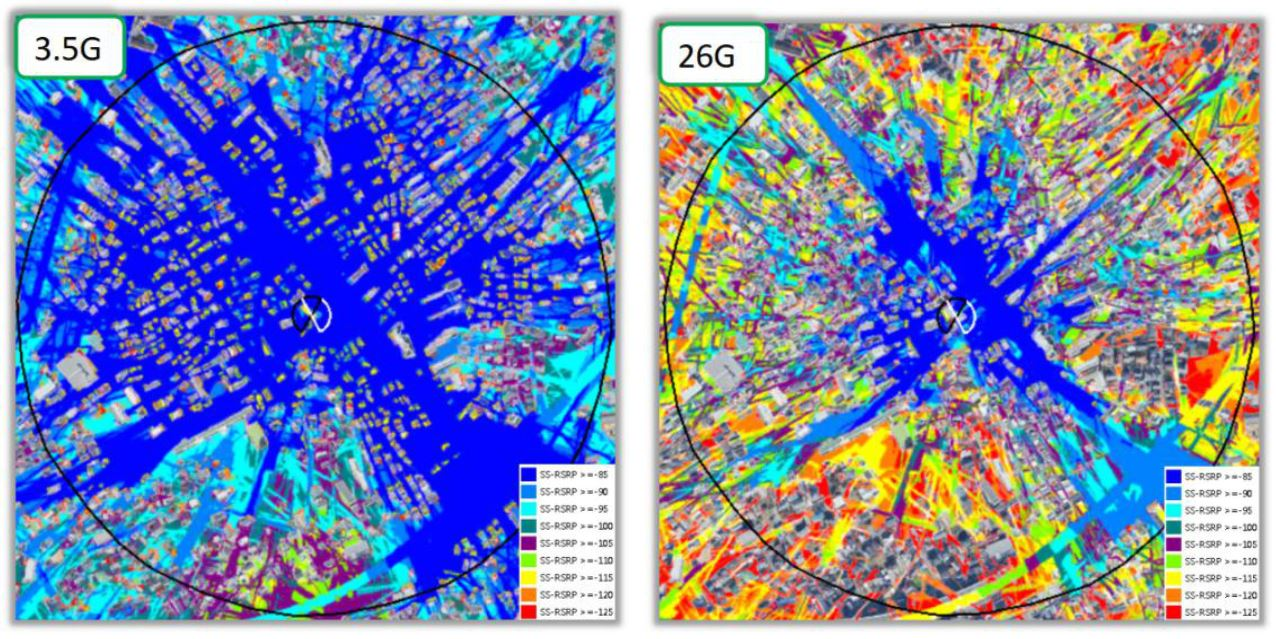
\includegraphics[width=0.8\linewidth]{Figures/Overlay-comparison.JPG}
\end{generalfig}

从毫米波设备的硬件架构来看,毫米波设备由大量的射频链路、射频开关、移相器组成用来实现模拟波束赋形。这样的收发器的组成需要所需的天线、放大器等器件相比现有通信方案增加多达数十倍,造成了成本长时间居高不下。
同时带来的也有能耗问题,复杂的射频硬件电路带来了令人难以置信的高功耗,这不是绿色通信的发展方向,也不利于实现碳中和(carbon neutrality)。

面对这些问题,急需一种能够规避高频信道不可靠性的方法,其中重要的一环便是能智能地改善当前的无线环境。
中继站是一种可以将非视距路径(Non-line-of-sight, NLoS)转化为视距路径的方法\cite{Dohler2010a}。
使用中继站传输时,需要为每个中继站配备专用的电源和射频前端,这需要很高的资本投入,而且,中继站需要先接收处理无线信号再做转发,会带来较大的时延,更为严重的是,广播出的新信号可能会干扰原信号\cite{di2020reconfigurable}。
反射阵列给出了有效的解决方案:当LoS径不能提供服务时,另一种建立替代路径的方法是通过无源非可重构镜面反射器。
反射阵列是指能够以波束的形式反射电磁波的平面\cite{huang2005reflectarray},这和曲面的反射镜不同,后者依靠物理曲率的变化决定反射波束的方向,而前者是由离散的单元组成,每个单元对应着不同的幅度和相移\cite{pozar1997design}。
无源非可重构的反射器与传统中继器相比,在成本和功耗方面有一定的优势。
但是,这种反射器的一个重大缺陷是它的反射在生产制造出来后就被固定了,在部署和使用是不可以修改的,这使得它无法适应高动态的无线信道环境。

近年来,人们研制出了能够对撞击的无线电波进行特定变换的基于电磁的可重构结构,它们的工作频段非常广阔,可以覆盖Sub-6 GHz、毫米波甚至太赫兹\cite{Wu2019}。下面将详细介绍这一新技术。

\subsection{智能超表面概述}

由于具有主动适应、改变无线通信环境的能力,可重构智能表面(RIS),也称为可重构反射阵列、可编程超表面、大型智能表面或智能反射表面,已成为无线通信研究领域的一个焦点,用于缓解在不同无线网络中遇到的各种挑战\cite{liu2020ris, huang2020holographic}。
智能超表面是由电磁材料构成的,因为它不需要改变现有的网络结构,也不需要修改现有的无线通信标准,所以特别适合“无感”地部署在建筑物外墙、公路指示牌、广告面板、车窗等平面物体上。
RIS能够通过被动反射接收信号在基站和移动用户之间形成虚拟视线链路,从而补偿长距离的功率损耗,智能地配置无线信号环境。
当基站和终端之间的直射链路被高层建筑阻断时,通过RIS的智能部署和设计,可以构建软件定义的无线环境,进而使接收信的信噪比(SINR)增强。
与传统放大转发和解码转发的中继系统相比,RIS不需要专用的大功率电源来运行,其功耗和硬件复杂度有着其他技术难以望其项背的优势\cite{di2020reconfigurable}。

2014年,中国科学院院士崔铁军教授首次提出了智能超表面并进行了实验验证,其基本结构如\autoref{fig:ris}所示\cite{cui2014coding}。
这是一种具有可编程电磁特性的二维薄层人工电磁表面结构,可以应用于从微波到可见光的各种波段中\cite{CHN_zhang2017}。
从\autoref{fig:ris}中可以看出,超表面由精心设计的电磁单元规则排列而成,这些电磁单元通常由金属铜片、电磁介质和可调元件\footnote{这里可调元件指的是变容二极管、PIN二极管、射频开关、MEMS器件等有不同状态的元件。}组成。
通过控制电磁单元中的可调元件,以可编程的方式更改反射的电磁波的电磁参数(例如幅度和相位)\cite{CHN_zhou2020}。

\begin{generalfig}[htb]{智能超表面示意图}{fig:ris}
	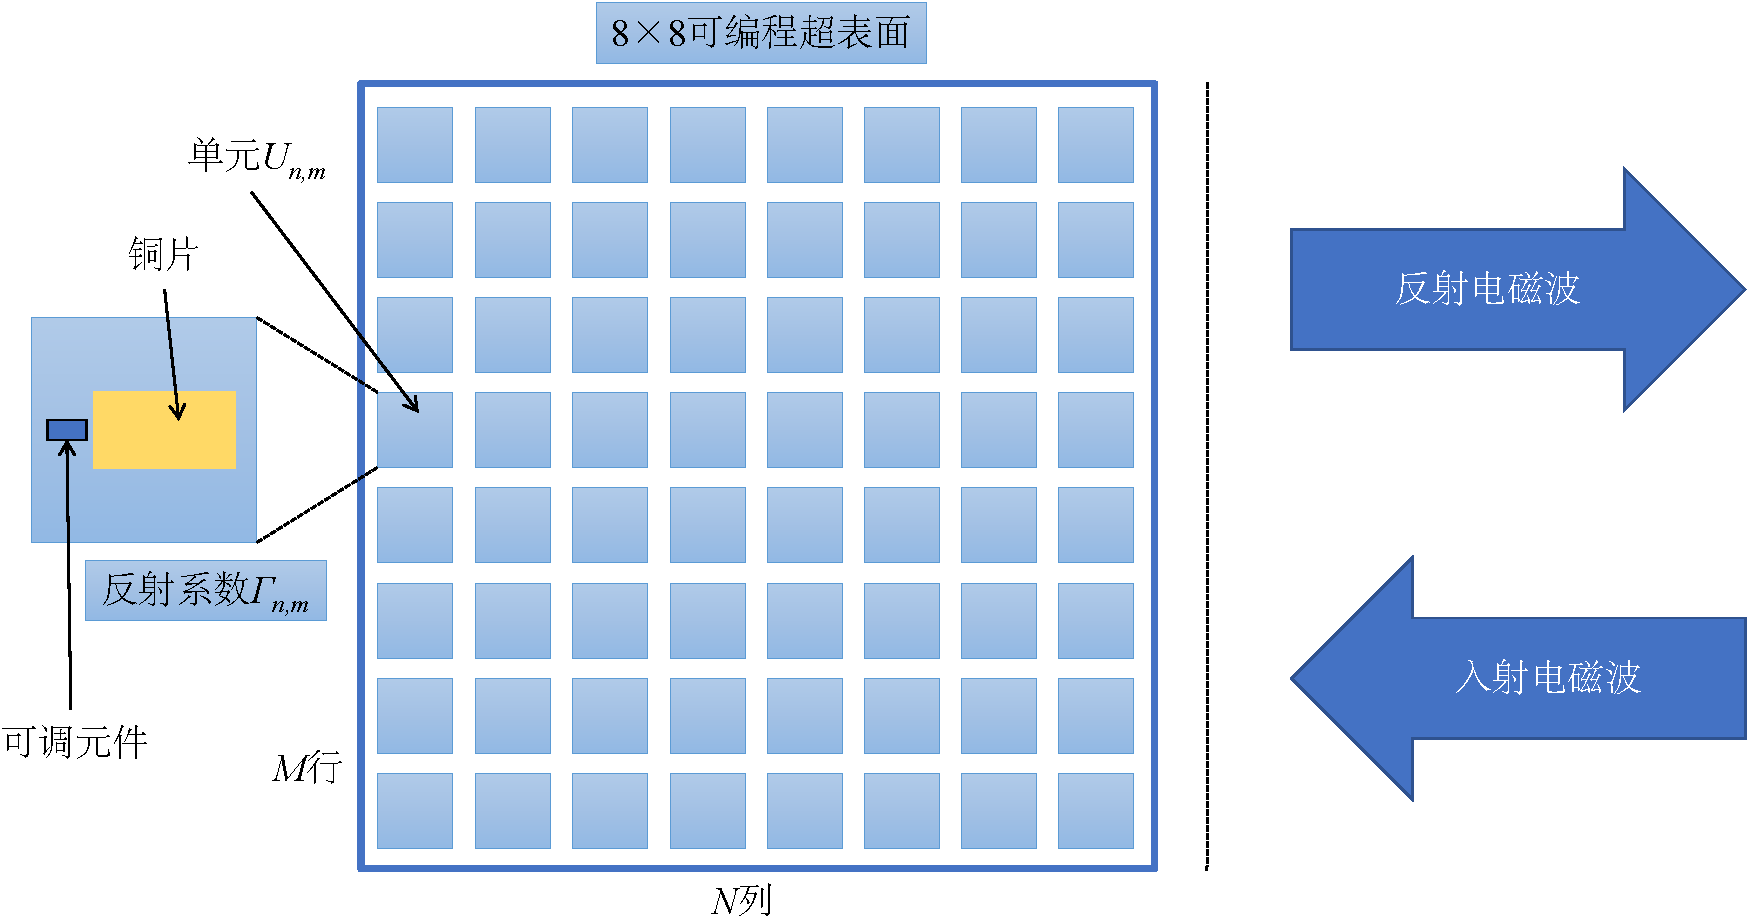
\includegraphics[width=0.8\linewidth]{Figures/ris.pdf}
\end{generalfig}

如\autoref{fig:Reflected-refracted}所示为智能超表面的异常反射、折射示意图,智能超表面可以将入射信号反射和折射到非斯涅尔定律预测的异常方向,可以改变入射电磁波的波形和极化方向\cite{Renzo2019}。
就无线电波的传播而言,基于超材料元表面的RIS就像一个突变的电磁间断,改变了散射场。
如前所述,实现智能超表面的功能的关键要素便是元表面单元结构的设计。
元表面是由亚波长金属或电介质散射粒子(称为亚原子)形成的亚波长阵列\cite{basar2019wireless}。
\autoref{fig:Reflected-refracted}描绘了电磁波对于给应的入射角,元表面的预期反射相应和折射相应,与普通平面的反射$ \theta_2 =  \theta_1 $不同,超表面可以使$ \theta_3 \ne \theta_1 $。

\begin{generalfig}[htb]{智能超表面的异常反射、折射}{fig:Reflected-refracted}
	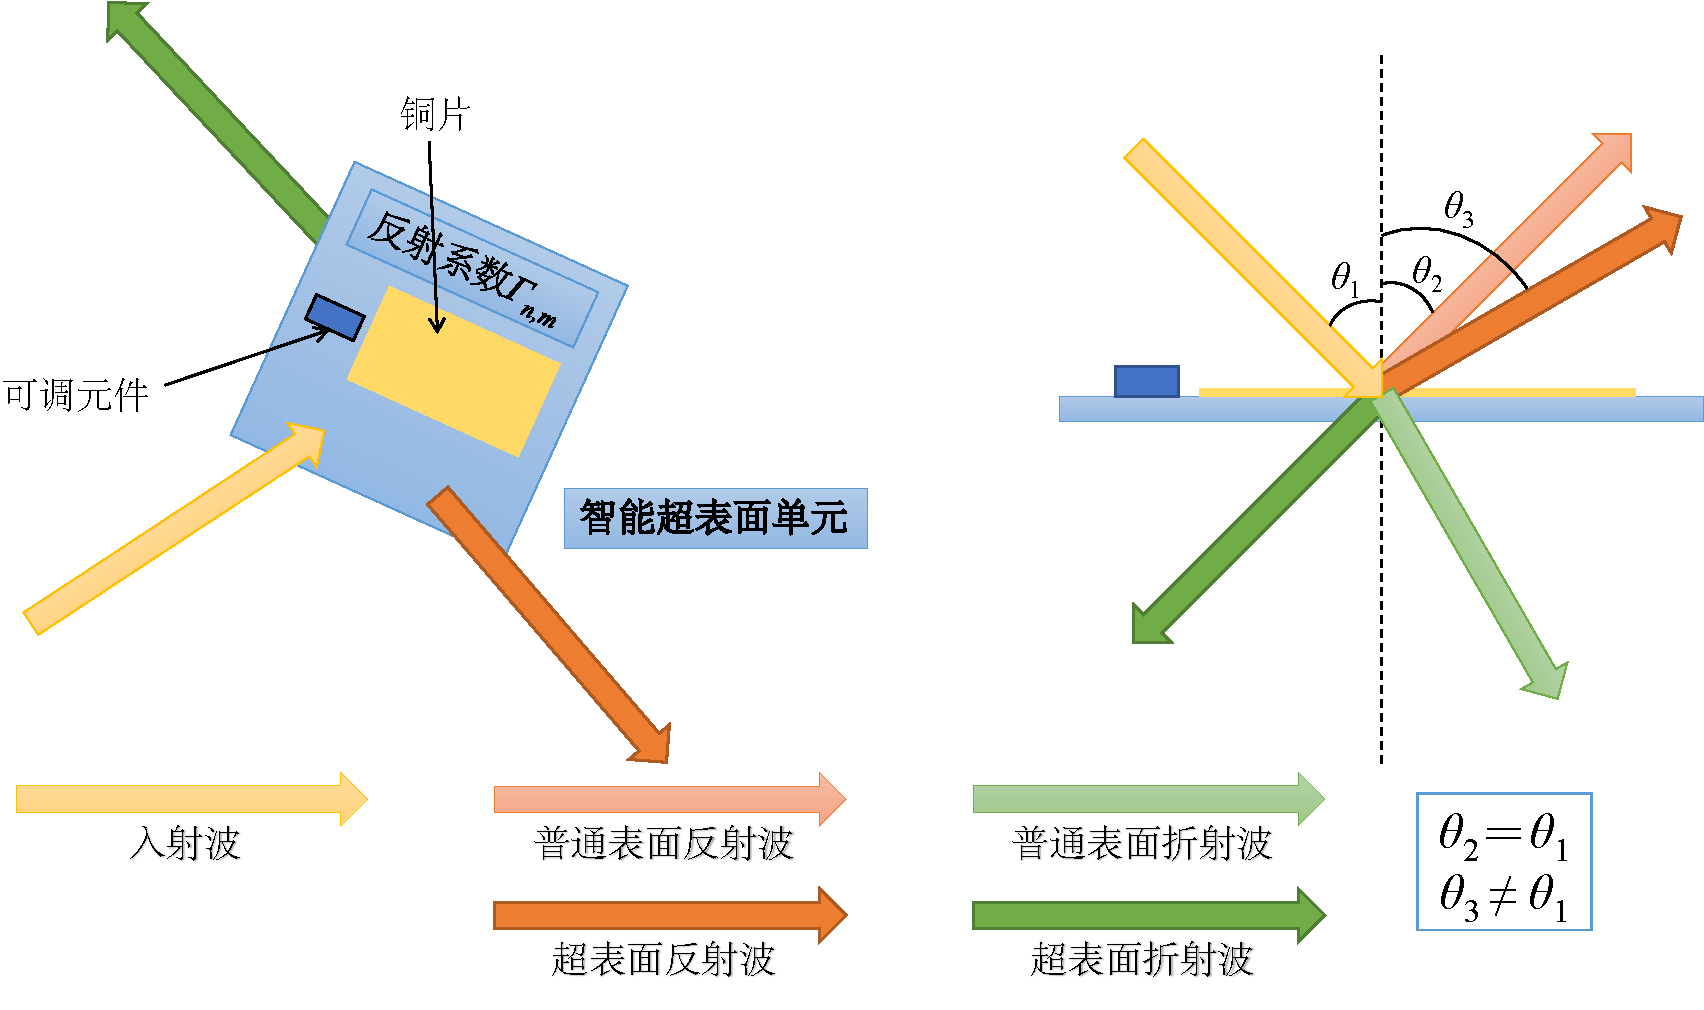
\includegraphics[width=0.8\linewidth]{Figures/Reflected-refracted.pdf}
\end{generalfig}

在智能超表面中,每个单元的反射系数$ \Gamma _ {n,m} $ 是可以根据外界环境调整改变的。
\autoref{fig:ris}上的可调元件一般被安装在单元上。
这样,通过外部的控制电路控制可调元件的状态,就可以操纵元表面上无线电波的波前,以实现信号调制或波束赋形。
智能超表面的中央控制器一般采用现场可编程逻辑门阵列(FPGA)或微控制器(MCU)。
通过软件设计,超表面可以实现对移动通信中电磁信号的实时调控。目前,国内外有关智能超表面在移动通信领域的研究主要集中在两个方向\cite{CHN_zhou2020},下面详细介绍国内外研究现状。

\subsection{国内外现状分析}


目前智能反射面的第一个主要研究方向是利用它进行无线中继,构建智能无线电环境。
如\autoref{fig:Ris-2way}(a)所示,RIS可以被认为是一个多功能的“神奇镜”,将它置于无线通信系统中,可以主动地改善无线传播环境,通过接收机的反馈动态调整反射系数,使得接收机处通过RIS反射和其他路径的叠加信号功率最大化,实现对电磁波资源的“再分配”。
国内外有许多RIS增强系统的主动和被动联合设计的研究:Qingqing Wu等人设计了在单用户和多用户情况下联合的主动和被动波束赋形,可以在接收用户SINR的约束下,最小化总发射功率\cite{Wu2019}。
智能超表面可以使得各个路径的波束在用户(UE)处相干增强,从而最大化接收功率。
Chongwen Huang等人将可重构智能表面用于多用户无线通信,他们通过设计RIS的相移和从基站到用户的功率分配策略,来最大化RIS系统的能效。
此外,文中还介绍了RIS的实际能耗模型。并针对基站发射功率分配和RIS反射系数提出了两个计算效率高的算法。
其中一种采用梯度下降方法设计,而另一种是基于分式规划方法。其中的仿真结果表明,与传统的多天线自动对焦中继相比,该系统能够获得高达300\%的能效\cite{Huang2018a}。

\begin{generalfig}[htb]{智能超表面的两大研究方向}{fig:Ris-2way}
	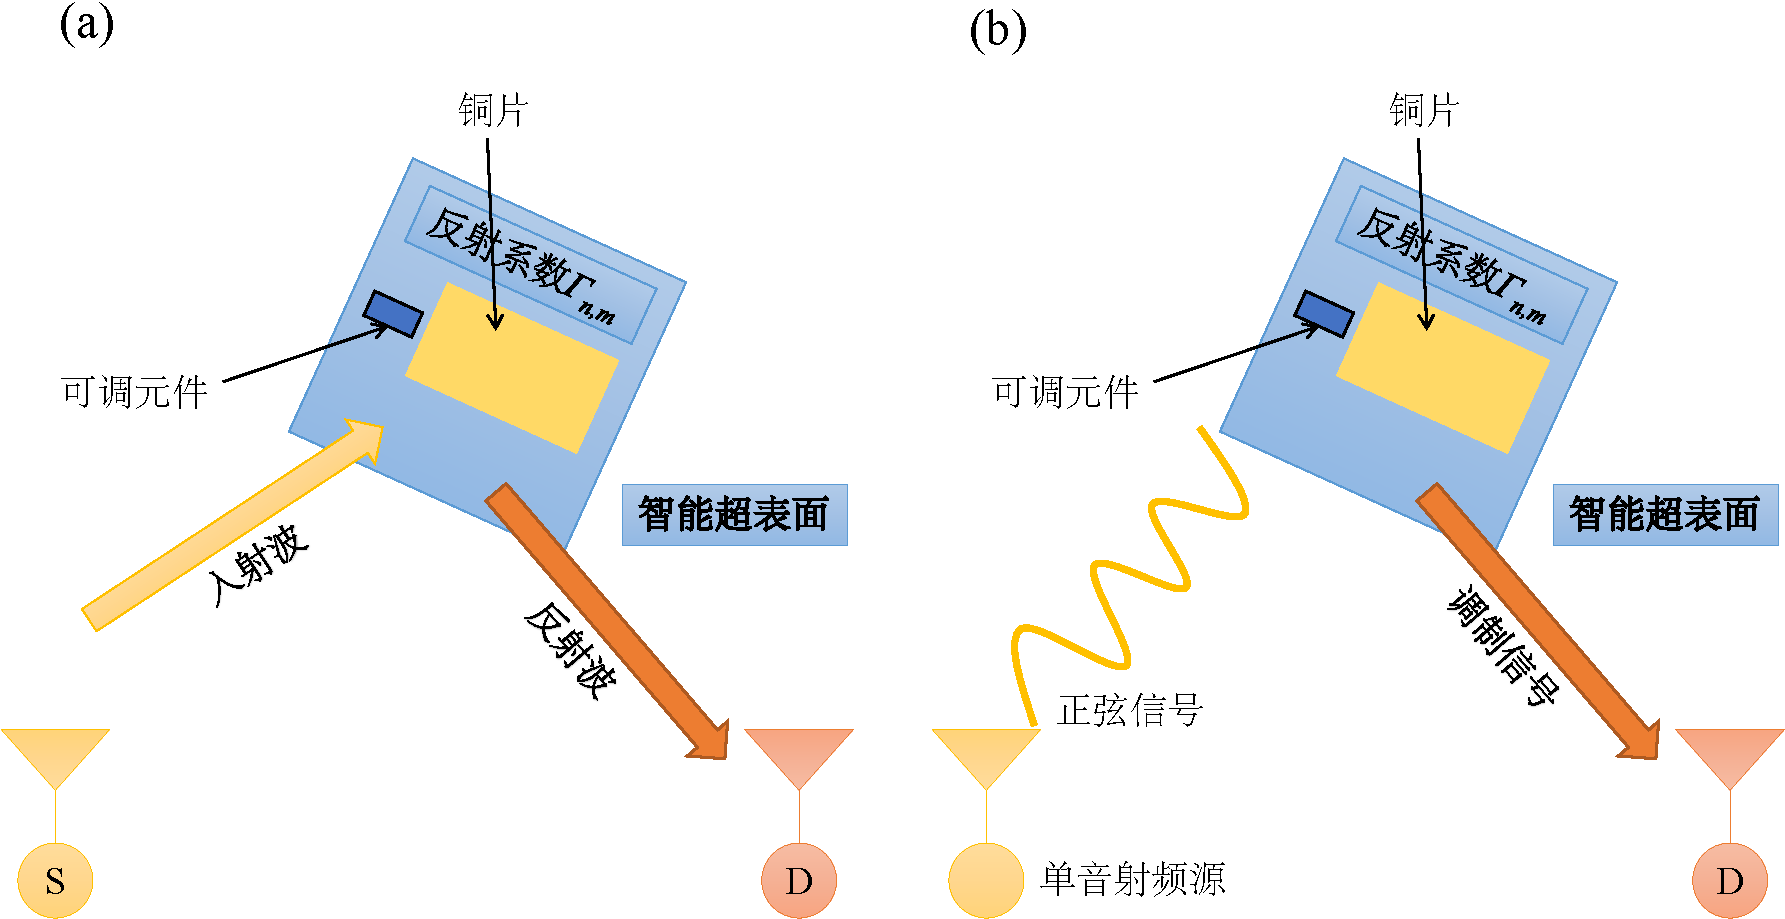
\includegraphics[width=0.8\linewidth]{Figures/Ris-2way.pdf}
\end{generalfig}

绝大多数的研究只停留在理论分析与建模仿真阶段,基于智能超表面的无线通信实验验证系统十分稀缺,目前只有少量的研究:
Zhuqi Li等人在室内环境中部署了一个$ 6 \times 6 $的可重构发射天线阵列,设计了信道分解算法来快速估计无线信道环境\cite{li2019towards}。通过实时配置无线信道,改善通信环境,系统的吞吐量提高到了原来的124\%。
2019年MIT研究团队展示了一个由3000多个无源天线组成的反射面(由几十块PCB板拼接而成),取名为“RFocus”,工作频率为1.6 GHz至3 GHz。
实验表明它可以使接收信号强度平均增加10.5倍,将信道容量平均提升两倍\cite{arun2019rfocus}。
2019年清华大学研究团队最近展示了一个工作在毫米波波段的$ 16 \times 16 $单元的智能超表面。
该RIS每个单元使用四个PIN二极管控制,可实现两比特的反射相位调整。这个系统实现了28.5 GHz下19.1 dBi的天线增益\cite{Dai2020}。

另外一个研究方向是通过智能超表面实现信号的编码与调制。
智能超表面可以灵活地调控电磁信号波前,改变诸如幅度、相位、频率甚至极化方向等电磁参数\cite{CHN_zhou2020}。
这一新型的发射机架构不需要复杂的基带信号处理和高性能的射频链路,未来有希望应用于毫米波通信和Massive MIMO系统中。
其基本结构如\autoref{fig:Ris-2way}(b)所示,基带信号直接作用于智能超表面,通过对反射系数的控制直接调制正弦信号。
东南大学崔铁军院士团队中提出了一种同时在时间和频率上操纵电磁波的时空调制数字可编程超表面,并实现了BFSK调制\cite{zhao2019programmable}。
进一步地,唐万凯等人设计了一个基于可编程表面的正交相移键控(QPSK)无线发射机的原型,实现了2.048 Mbit/s的数据传输速率,视频流也能实时传输\cite{Tang2019Wireless}。

\subsection{本文主要研究内容与组织结构安排}
todo
本文的主要研究内容是如何利用可编程电磁超表面增强5G信号覆盖。
文中首先在\autoref{sec:theory}介绍了电磁超表面的相关基础理论,包括广义反射定律和折射定律以及波束赋形理论。

\autoref{sec:simulation}开始对RIS通信系统建模分析,比较了巴拉巴拉

\autoref{sec:design}设计了一个由可编程超表面及其控制电路构成的智能反射面系统,

最后,在\autoref{sec:conclusion}得出结论,并对未来的研究工作作了初步分析。

\section{超表面基础理论}\label{sec:theory}

超表面和超材料有着完善复杂的理论,本章根据后续内容的需要着重介绍广义斯涅尔定律和超表面对电磁信号的调控机理。

\subsection{广义反射和折射定律}\label{subsec:snell-law}

电磁波在超表面上会发生相位或幅度的突变,这一现象的理论依据是广义斯涅尔定律\cite{9326394}。
2011年Capasso教授等人发现了相位不连续的电磁波传播,并提出了广义反射和折射定律\cite{yu2011light}。
通过沿着电磁波传播路径,在波长范围内引入突变相移,可以获得控制波前的新自由度。
费马原理指出光线在两点A和B之间的轨迹是最小光程的轨迹,即$ \int_{A}^{B} n(\vec{r}) dr $,其中$ n(\vec{r}) $是局部折射率,由此容易推演得到两种介质之间的反射和折射定律。
在其最普遍的形式中,费马原理可以表述为固定相原理\cite{feynman2010quantum},也就是说,相对于路径的无穷小变化,沿着实际光路累积的相位导数$ \int_{A}^{B} d \varphi (\vec{r}) $将为零。
但是研究表明,通过适当设计两种介质之间的界面,可以在光路中引入波长范围内的突然相移$ \Phi (\vec{r}_\mathrm{s}) $,相移$ \Phi (\vec{r}_\mathrm{s}) $取决于沿界面的坐标$ \vec{r}_\mathrm{s} $。
那么,对于光所走的实际路径,总相移$ \Phi\left(\vec{r}_{\mathrm{s}}\right)+\int_{A}^{B} \vec{k} \cdot d \vec{r} $是固定不变的,其中$ \vec{k} $是传播光的波矢。
这提供了反射和折射定律的一般化,其适用于整个光谱中两种介质之间的大范围的亚波长结构化界面。

\begin{generalfig}[htb]{广义斯涅尔折射定律的示意图}{fig:Snell-Law}
	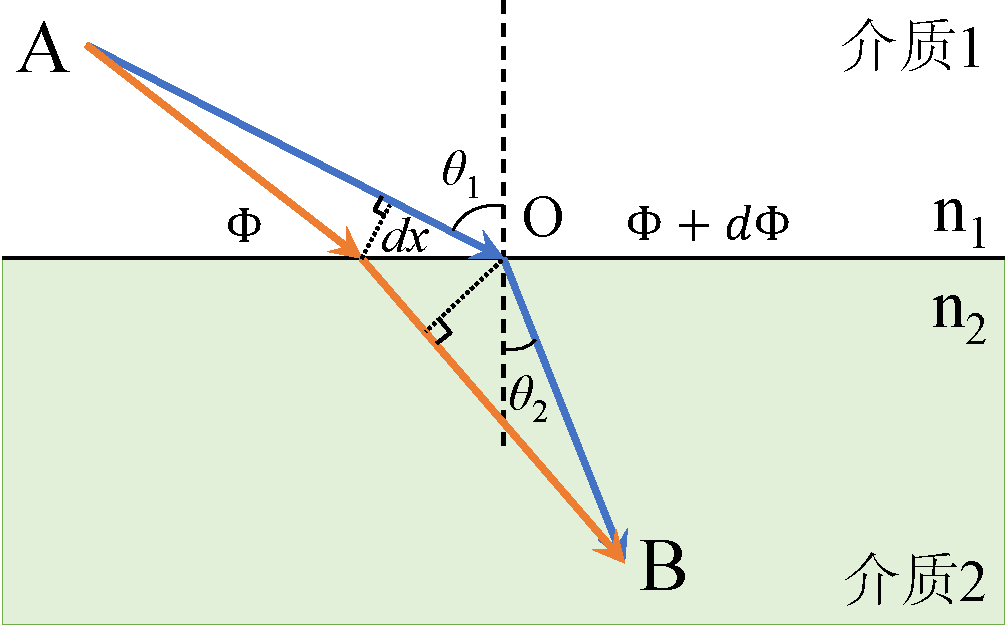
\includegraphics[width=0.5\linewidth]{Figures/Snell-Law.pdf}
\end{generalfig}

下面考虑{\bfseries 广义反射和折射定律},在两种介质的界面上引入一个突变的相移,称为相位不连续,这使得我们可以通过应用费马原理来重新审视反射和折射定律。
\autoref{fig:Snell-Law}中的入射平面波入射角为$\theta_1$,假设两条光路无限接近实际光路,那么它们之间的相位差为零,有:
\begin{equation}
	k_\mathrm{o} n_1 \sin (\theta_1) dx + (\Phi + d\Phi) = k_\mathrm{o} n_2 \sin (\theta_2) dx + \Phi
	\label{eq:Generalized-snell-law-pre}
\end{equation}
其中$ \theta_2 $为折射角,$ \Phi $和$ \Phi + d\Phi $分别是两条路径穿过界面位置处的相位不连续性,$ dx $是两条路径界面处的距离差,$n_1$是上层介质的折射率,$n_2$为下层介质的折射率,$k_\mathrm{o}=2 \pi / \lambda_\mathrm{o}$,$\lambda_\mathrm{o}$为真空中的光波波长。

如果沿界面的相位梯度被设计为常数,由\autoref{eq:Generalized-snell-law-pre}可以推导出广义的斯涅尔折射定律:
\begin{equation}
	n_2 \sin \theta_2 - n_1 \sin \theta_1 = \frac{1}{k_\mathrm{o}} \frac{d \Phi}{dx}
	\label{eq:Generalized-snell-law}
\end{equation}
\autoref{eq:Generalized-snell-law}意味着折射光束可以具有任意方向,只要沿界面引入相位不连续性的合适的恒定梯度$d\Phi/dx$。
由于在\autoref{eq:Generalized-snell-law}中引入了非零的相位梯度$d\Phi/dx$,两个入射角$\pm \theta_1$会导致不同的折射角。
因此,全内反射在$n_2<n_1$时有两种可能的临界角:
\begin{equation}
	\theta_{\mathrm{c}}=\arcsin \left(\pm \frac{n_{2}}{n_{1}}-\frac{\lambda_{\mathrm{o}}}{2 \pi n_{1}} \frac{d \Phi}{d x}\right)
\end{equation}

同理,由\autoref{eq:Generalized-snell-law}也可以推导出广义斯涅尔反射定律。对于反射的情况,入射波和反射波都在介质1中,所以有$n_2=n_1$,可得:
\begin{equation}
	\sin \theta_2 - \sin \theta_1 = \frac{1}{k_\mathrm{o} n_1} \frac{d \Phi}{dx}
	\label{eq:Generalized-snell-law-reflection}
\end{equation}
此时$\theta_2$是反射角,入射角$\theta_1$和反射角$\theta_2$之间存在非线性关系,这与传统的镜面反射明显不同。
由\autoref{eq:Generalized-snell-law-reflection}可知总有一个临界角$\theta_{\mathrm{c}}^{\prime}$满足:
\begin{equation}
	\theta_{\mathrm{c}}^{\prime}=\arcsin \left(1-\frac{\lambda_{\mathrm{o}}}{2 \pi n_{1}}\left|\frac{d \Phi}{d x}\right|\right)
\end{equation}
在入射角$\theta_1 = \theta_{\mathrm{c}}^{\prime}$时,反射波束将不存在。

广义反射和折射定律可以统一写成如下的形式\cite{ding2017gradient}:
\begin{eqnarray}
	k_{x}^{(r)}-k_{x}^{(i)}=\frac{d \Phi}{d x} \\
	k_{x}^{(t)}-k_{x}^{(i)}=\frac{d \Phi}{d x}
\end{eqnarray}
其中$k_{x}^{(i, r, t)}=k_{\mathrm{o}} n_{i, i, t} \sin \theta_{i, r, t}$表示平面波矢量。标号$i$表示入射侧的参量,标号$r$表示反射侧的参量,标号$t$表示折射侧的参量。
当$\frac{d \Phi}{d x}=0$时,即得到经典的斯涅尔定律。

广义斯涅尔定律为超表面的设计提供了理论指导,在设计超表面的过程中,我们只需要将它分解为二维亚波长单元,分析每个单元对电磁波带来的附加相位,通过对反射阵列的附加相位的设计,结合波束赋形理论,就可以实现对电磁波的灵活调控。

\subsection{超表面对电磁波的调控机理}

todo



\subsection{本章小结}

本章主要介绍了

\section{物理、传播和路径损耗建模}\label{sec:modeling}

本章中,我们使用物理光学知识导出了远场路径损耗\cite{emil2019intelligent},并解释了为什么智能超表面由许多元素组成,这些元素单独充当散射体,但可以在特定波束宽度的期望方向上联合波束赋形。本章首先将从无源金属表面的散射分析引入。

\subsection{无源金属表面}\label{subsec:metal-plate}

在这一节中,我们总结了由有限尺寸的无源的完全导电的金属板散射的波形的场强和波束宽度的研究。这些结果将被用来解释智能超表面的理想工作状态。

我们考虑一个尺寸为$a \times b$的厚度可以忽略的矩形完美导电板,且位于水平面上(即$\boldsymbol{e}_{x}, \boldsymbol{e}_{y}$所在平面)。一个距离为$d_i$的很远的点源辐射具有波数为$k$($k = 2\pi / \lambda$,$\lambda$为波长)的线性极化电磁波。
为了便于讨论,我们假设源的极化是这样的,即电场平行于$\boldsymbol{e}_{x}$,而磁场位于$\boldsymbol{e}_{y}, \boldsymbol{e}_{z}$所跨越的平面上。
$\theta_{i} \in\left[0, \frac{\pi}{2}\right]$表示为入射角,即电磁波的坡印亭矢量与$\boldsymbol{e}_{z}$的夹角,$\theta_{s}$为散射角,如\autoref{fig:metal-plate}所示。

\begin{generalfig}[htb]{入射波被金属板散射示意图}{fig:metal-plate}
	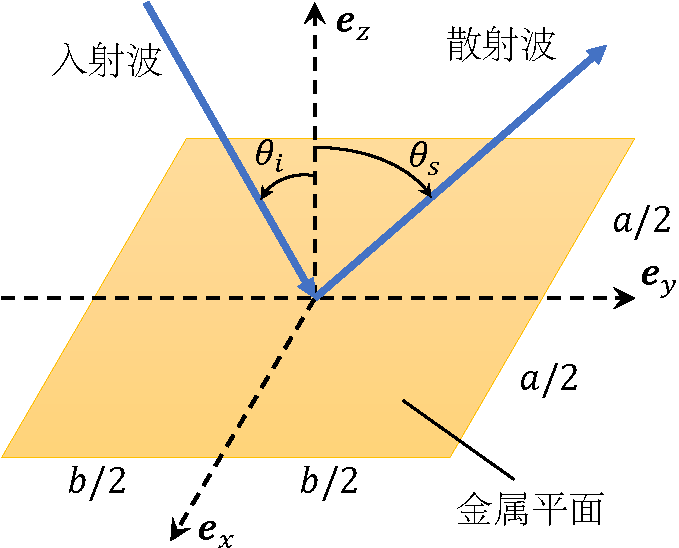
\includegraphics[width=0.5\linewidth]{Figures/metal-plate.pdf}
\end{generalfig}

进一步假设,相对于金属板的尺寸,$d_i$足够大,符合远场模型。此时入射波为幅度为$E_i$的平面波。
这时入射的平面波的电场和磁场分布可以表示为:
\begin{equation}
	\begin{array}{l}
		\mathbf{E}_{i}=E_{i} e^{-j k\left(\sin \left(\theta_{i}\right) y-\cos \left(\theta_{i}\right) z\right)} \boldsymbol{e}_{x} \\
		\mathbf{H}_{i}=-\frac{E_{i}}{\eta}\left(\cos \left(\theta_{i}\right) \boldsymbol{e}_{y}+\sin \left(\theta_{i}\right) \boldsymbol{e}_{z}\right) e^{-j k\left(\sin \left(\theta_{i}\right) y-\cos \left(\theta_{i}\right) z\right)}
	\end{array}
	\label{eq:e-field}
\end{equation}
其中$\eta$是介质的特征阻抗。

电场会引起电子在金属板中的运动。
由于电场与$\boldsymbol{e}_{y}$正交,电子将沿$\boldsymbol{e}_{x}$方向移动,而不会沿$\boldsymbol{e}_{y}$方向移动。
因为金属板的厚度忽略不计,电子也不会沿$\boldsymbol{e}_{z}$方向移动。
运动的电子感应电磁辐射,产生散射波。

\begin{lemma}
	\label{lemma:scattered-field}
	在$\boldsymbol{e}_{y}, \boldsymbol{e}_{z}$平面内,对于任意观察角度$\theta_{s} \in\left[0, \frac{\pi}{2}\right]$(相对于$\boldsymbol{e}_{z}$),在远场观察距离$r \geq \frac{2 \max \left(a^{2}, b^{2}\right)}{\lambda}$时,散射场的平方幅度为:
	\begin{equation}
		S\left(r, \theta_{s}\right)=\left(\frac{a b}{\lambda}\right)^{2} \frac{E_{i}^{2}}{r^{2}} \cos ^{2}\left(\theta_{i}\right)\left(\frac{\sin \left(\frac{\pi b}{\lambda}\left(\sin \left(\theta_{s}\right)-\sin \left(\theta_{i}\right)\right)\right)}{\frac{\pi b}{\lambda}\left(\sin \left(\theta_{s}\right)-\sin \left(\theta_{i}\right)\right)}\right)^{2}
		\label{eq:scattered-field}
	\end{equation}
\end{lemma}

\begin{proof}
	这个结果来自标准的物理光学技术(忽略边缘效应)\cite{balanis2012advanced}。
\end{proof}

从\autoref{eq:scattered-field}中关于散射场的平方幅度的公式可以发现,对于我们考虑的极化方式来说,当观察角度$\theta_{s}=\theta_{i}$即镜面反射时,$S\left(r, \theta_{s}\right)$达到最大值,这和斯涅尔反射定律所描述的是吻合的。

\subsubsection{散射波的波束宽度}

\autoref{eq:scattered-field}揭示了散射场就像是一个波束,随着$\theta_{s}$远离$\theta_{i}$,强度越来越弱。在\normalcite{emil2019intelligent}中,作者运用三角函数和泰勒展开的数学知识推导出散射波的$-3\,\mathrm{dB}$宽度为:
\begin{equation}
	2\left|\theta_{s}-\theta_{i}\right|<2\sqrt{\frac{1}{2} \frac{3 \lambda^{2}}{\pi^{2} b^{2} \cos ^{2}\left(\theta_{i}\right)}}=2\sqrt{\frac{3}{2}} \frac{\lambda}{\pi b \cos \left(\theta_{i}\right)}
\end{equation}

这个不等式表明,$-3\,\mathrm{dB}$的波束宽度与金属板板宽$b$成反比。波束宽度也与波长$\lambda$成正比,因此普通尺寸的板可以在可见光谱中提供非常窄的波束宽度,就像一束光照射在镜子上一样。
但是在典型的无线电光谱波段中,波束宽度要宽四至五个数量级。

\subsubsection{多个相邻金属表面}

由于单个金属板的尺寸有限,有时可以部署多个相邻的板。
如果板子之间的间隙足够大,那么耦合效应可以忽略。
当来自不同的金属板的散射场在给定位置被接收时,相对的相移将导致干涉相长或干涉相消。
在理想的干涉相长下,来自$N$个平板的平方场强为:
\begin{equation}
	\left(N \sqrt{S\left(r, \theta_{s}\right)}\right)^{2}=N^{2} S\left(r, \theta_{s}\right)
	\label{eq:Multiple-Metallic-Surfaces}
\end{equation}

\autoref{eq:Multiple-Metallic-Surfaces}表明,只要总面积确定,无论是由许多小的还是几个大的金属板组成,最大接收功率是相同的。

\subsection{智能超表面的系统模型}

智能超表面的主要目的是实现“异常反射”\cite{liang2015anomalous},这意味着对散射场进行整形,使主波束指向接收器。考虑一个由与\autoref{fig:metal-plate}相同尺寸的超表面和相同的撞击平面波组成的反射系统。RIS的目标是实现全反射,并将主光束指向我期望方向$\theta_r$。
因此,超表面必须被设计成获得反射或散射波的以下理想场分布:
\begin{equation}
	\begin{array}{l}
		\mathbf{E}_{r}=E_{r} e^{-j k\left(\sin \left(\theta_{r}\right) y+\cos \left(\theta_{r}\right) z\right)} \boldsymbol{e}_{x} \\
		\mathbf{H}_{r}=-\frac{E_{r}}{\eta}\left(\sin \left(\theta_{r}\right) \boldsymbol{e}_{z}-\cos \left(\theta_{r}\right) \boldsymbol{e}_{y}\right) e^{-j k\left(\sin \left(\theta_{r}\right) y+\cos \left(\theta_{r}\right) z\right)}
	\end{array}
\end{equation}

使用\autoref{subsec:snell-law}中介绍的广义斯涅尔定律,利用\autoref{eq:Generalized-snell-law-reflection},可以通过调整超表面相位分布或表面阻抗将入射波$\left(\mathbf{E}_{i}, \mathbf{H}_{i}\right)$转换成散射波$\left(\mathbf{E}_{r}, \mathbf{H}_{r}\right)$。
在超表面上$(z = 0)$,入射和反射电场的叠加可以写成\cite{Asadchy_2016}:
\begin{equation}
	\mathbf{E}_{t}=E_{i} e^{-j k \sin \left(\theta_{i}\right) y} \boldsymbol{e}_{x}+E_{r} e^{-j k \sin \left(\theta_{r}\right) y} \boldsymbol{e}_{x}
\end{equation}
由此可得,期望反射系数的期望相位是:
\begin{equation}
	\phi_{r}(y)=\angle\left(\frac{E_{r} e^{-j k \sin \left(\theta_{r}\right) y}}{E_{i} e^{-j k \sin \left(\theta_{i}\right) y}}\right)=-k \sin \left(\theta_{r}\right) y+k \sin \left(\theta_{i}\right) y
\end{equation}
并且对$y$进行微分给出了广义斯内尔定律中反射系数的梯度:
\begin{equation}
	k\left(\sin \left(\theta_{i}\right)-\sin \left(\theta_{r}\right)\right)=\frac{d \phi_{r}(y)}{d y}
\end{equation}
它给出了$\theta_i,\theta_r$和局部表面相位$\phi_{r}(y)$之间的关系。

\subsubsection{传播和路径损耗模型}

与单纯的金属表面不同,智能超表面必须由许多小单元组成,细致的配置每个单元的相位,可以获得角度为$\theta_r$的主反射波束。
如\autoref{subsec:metal-plate}中所述,\autoref{eq:e-field}中的入射波电场在$\boldsymbol{e}_{x}$方向上感应出表面电流。
通过调整每个元件的表面阻抗,调整该电流,以获得近似广义斯内尔定律所需的表面相位分布。

\begin{lemma}
	当使用智能超表面向$\theta_r$方向反射信号时,任意观察角度$\theta_{s} \in\left[-\frac{\pi}{2}, \frac{\pi}{2}\right]$下,在远场观察距离$r \geq \frac{2 \max \left(a^{2}, b^{2}\right)}{\lambda}$时,散射场平方幅度为:
	\begin{equation}
		S_{\mathrm{IRS}}\left(r, \theta_{s}, E_{i}^{2}\right) =\left(\frac{a b}{\lambda}\right)^{2} \frac{E_{i}^{2} \cos ^{2}\left(\theta_{i}\right)}{r^{2}}\left(\frac{\sin \left(\frac{\pi b}{\lambda}\left(\sin \left(\theta_{s}\right)-\sin \left(\theta_{r}\right)\right)\right)}{\frac{\pi b}{\lambda}\left(\sin \left(\theta_{s}\right)-\sin \left(\theta_{r}\right)\right)}\right)^{2}
	\end{equation}
\end{lemma}

\begin{proof}
	超表面的厚度可以忽略不计,这使得我们可以写出超表面上某处$(z=0, y=y^\prime)$的电流密度$J_{x}=\frac{2 E_{i}}{\eta} \cos \left(\theta_{i}\right) e^{-j k \sin \left(\theta_{r}\right) y^{\prime}}$。假设超表面是无损的,上述引理利用引理~\ref{lemma:scattered-field}可以证明。
\end{proof}

假设基站端的发射机发射功率为$P_t$,发射天线的增益为$G_t$,$E_i$和$P_t$之间的关系可以表示为:
\begin{equation}
	\frac{E_{i}^{2}}{2 \eta}=\frac{P_{t} G_{t}}{4 \pi d_{i}^{2}}
\end{equation}
此外,假设接收器天线的有效面积为$\frac{\lambda^2}{4\pi} G_r$,其中$G_r$为接收天线的增益。可得,距离为$r$时,在方向$\theta_r$上,接收信号功率$P_r$为:
\begin{equation}
	P_{r}\left(P_{t}, d_{i}, r, \theta_{s}\right)=\frac{1}{2 \eta} S_{\mathrm{IRS}}\left(r, \theta_{s}, \frac{P_{t} G_{t} \eta}{2 \pi d_{i}^{2}}\right)\left(\frac{\lambda^{2}}{4 \pi} G_{r}\right)
\end{equation}

\begin{corollary}
	当使用智能超表面向$\theta_r$方向上反射电磁波时,远场距离为$r$时的路径损耗是:
	\begin{equation}
		\begin{array}{l}
			\beta_{\mathrm{IRS}}\left(r, d_{i}, \theta_{s}\right)=\frac{P_{r}\left(P_{t}, d_{i}, r, \theta_{s}\right)}{P_{t}} \\
			=\frac{G_{t} G_{r}}{(4 \pi)^{2}}\left(\frac{a b}{d_{i} r}\right)^{2} \cos ^{2}\left(\theta_{i}\right)\left(\frac{\sin \left(\frac{\pi b}{\lambda}\left(\sin \left(\theta_{s}\right)-\sin \left(\theta_{r}\right)\right)\right)}{\frac{\pi b}{\lambda}\left(\sin \left(\theta_{s}\right)-\sin \left(\theta_{r}\right)\right)}\right)^{2}
		\end{array}
	\end{equation}

	当接收机处于理想位置时,即$\theta_s=\theta_r$,路径损耗简化为:
	\begin{equation}
		\beta_{\mathrm{IRS}}\left(r, d_{i}, \theta_{r}\right)=\frac{G_{t} G_{r}}{(4 \pi)^{2}}\left(\frac{a b}{d_{i} r}\right)^{2} \cos ^{2}\left(\theta_{i}\right)
	\end{equation}
\end{corollary}

\subsubsection{智能超表面的散射体阵列模型}

\subsubsection{智能超表面的传输系统模型}

考虑直射径下发射机和接收机之间的信道为$\sqrt{\beta_{\mathrm{sd}}} e^{j \phi_{\mathrm{sd}}}$,囊括智能超表面的反射路径,接收信号可以表示为:
\begin{equation}
	y=\left(\sqrt{\beta_{\mathrm{IRS}}^{s}} \mathbf{h}_{\mathrm{sr}}^{\mathrm{T}} \boldsymbol{\Theta} \mathbf{h}_{\mathrm{rd}}+\sqrt{\beta_{\mathrm{sd}}} e^{j \phi_{\mathrm{sd}}}\right) x+n
\end{equation}

在这封信中,我们首先在第二节解释了无源金属表面如何散射入射波,然后在第三节推导出红外反射器必须如何设计来模拟这种表面,同时控制散射波的方向性,从而填补了这一空白。这就产生了一个严格的路径损耗模型,以及一种建立可用于进一步研究的系统模型的方法。



\section{系统传输建模仿真分析}\label{sec:simulation}

\subsection{系统模型}

考虑从单天线源到单天线目的地的通信(SISO)。确定性平坦衰落信道表示为$h_{\mathrm{sd}} \in \mathbb{C}$,目的地接收到的信号是:
\begin{equation}
	y=h_{\mathrm{sd}} \sqrt{p} s+n
\end{equation}
其中$p$是发射功率,$s$是单位功率信息信号,$n \sim \mathcal{N}_{\mathbb{C}}\left(0, \sigma^{2}\right)$是接收机噪声。为了便于分析,天线增益包含在信道中。
该单输入单输出(SISO)信道的容量为:
\begin{equation}
	R_{\mathrm{SISO}}=\log _{2}\left(1+\frac{p\left|h_{\mathrm{sd}}\right|^{2}}{\sigma^{2}}\right)
\end{equation}
通过在通信中加入额外的设备,可以潜在地增加容量。

在本章中,我们考虑两种不同的中继方式,其一为智能超表面,其二为中继器。智能超表面被配置为使反射波束指向目的地,中继器工作于经典的解码转发模式下。
下面导出相应的可实现速率,然后通过分析进行优化,以实现公平的比较。
然而,本章中选择的信道模型是“偏心”智能超表面的,特别是确定性平坦衰落信道的假设对于智能超表面辅助增强通信是理想的,因为它不能获取信道状态信息(Channel State Information, CSI),比中继站更不能处理信道估计和频率选择性衰落。

\subsubsection{智能超表面使能的传输}

如图xxxxxx(a)所示,RIS由总共由$L$个元素组成。从基站到智能超表面的确定性信道表示为$\mathbf{h}_{\mathrm{sr}} \in \mathbb{C}^{L}$,$\left[\mathbf{h}_{\mathrm{sr}}\right]_{l}$代表第$l$个结构单元的信道。从智能超表面到终端的信道表示为$\mathbf{h}_{\mathrm{rd}} \in \mathbb{C}^{L}$,每个单元的尺寸都小于入射波波长,这样可以认为\cite{emil2019intelligent}

因此,它以近似恒定的增益向所有感兴趣的方向散射输入信号


\subsection{分析性能比较}
\subsection{仿真性能比较}
\subsection{本章小结}

本章

\section{系统设计与实现}\label{sec:design}

\subsection{智能超表面选择}\label{subsec:28-GHz-RIS}

本设计选用了\autoref{fig:28-GHz-RIS}所示的工作频点为28 GHz的智能超表面。
其中\autoref{fig:28-GHz-RIS}(a)为三维仿真图,\autoref{fig:28-GHz-RIS}(b)为实物图。

\begin{figure}[htb]
	\centering
	\subfloat[三维仿真图]{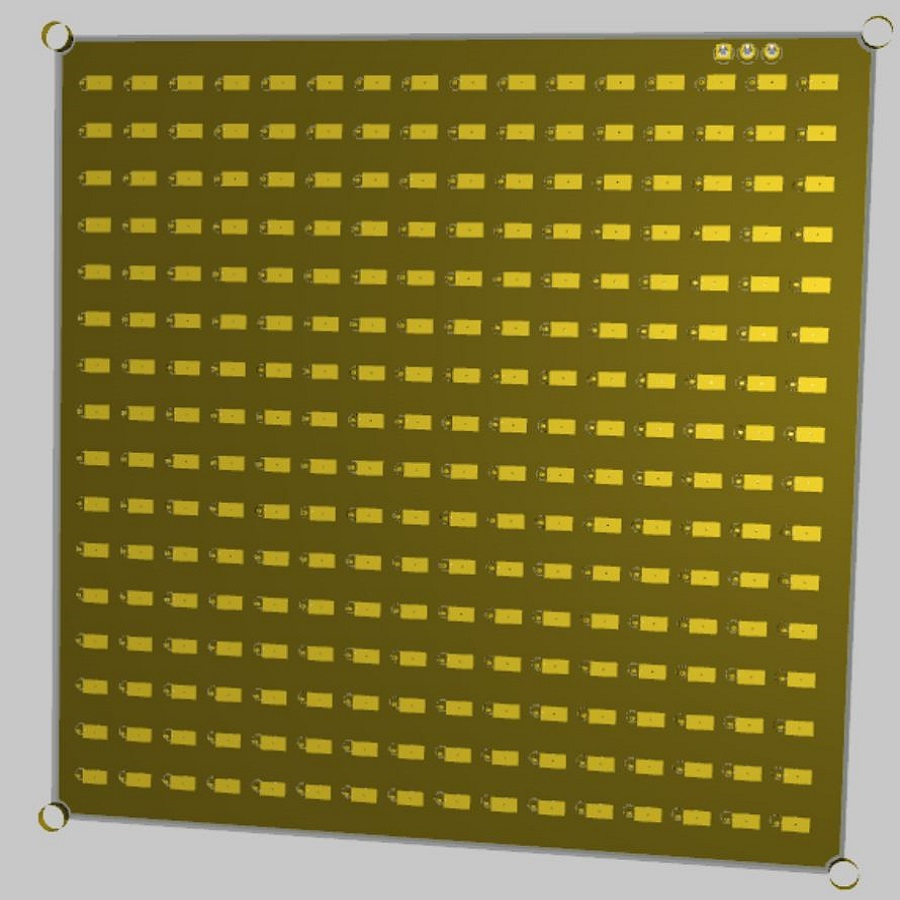
\includegraphics[width=0.3\linewidth]{Figures/28-GHz-RIS-3D.JPG}}
	\hfil
	\subfloat[实物图]{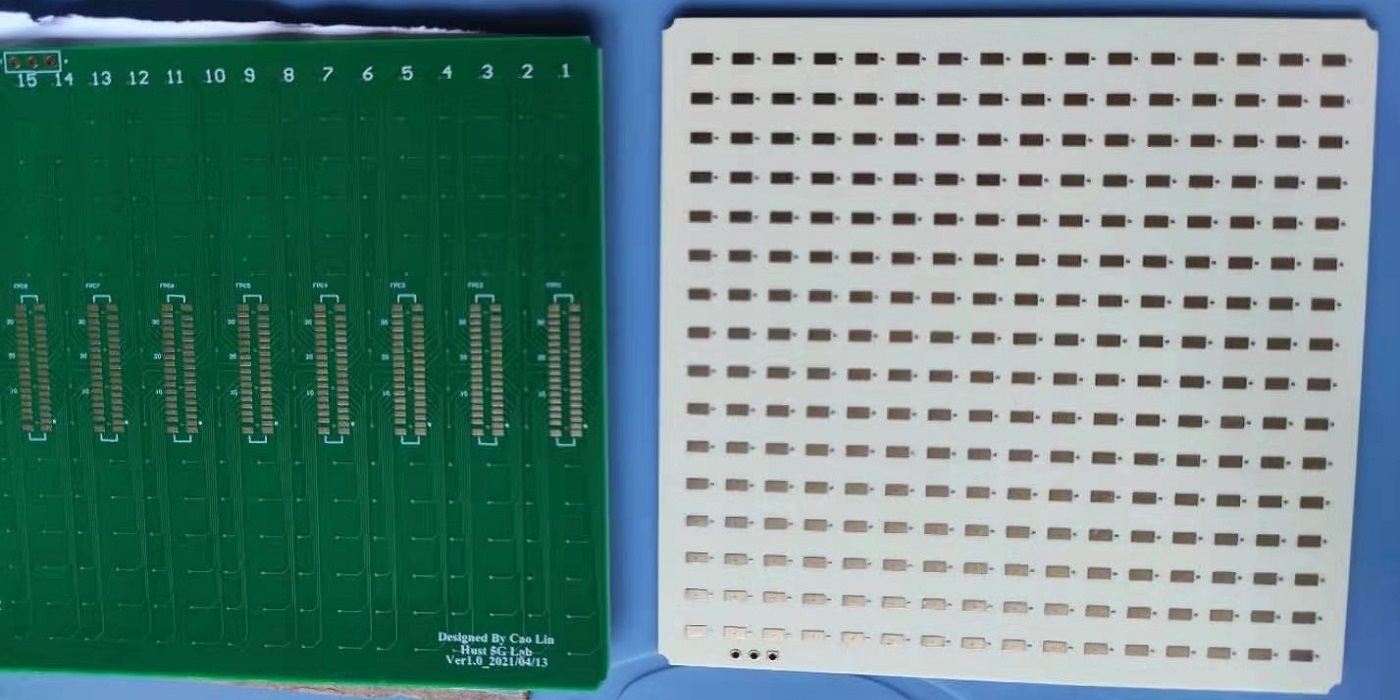
\includegraphics[width=0.6\linewidth]{Figures/28-GHz-RIS-real.jpg}}
	\caption{28 GHz智能超表面}
	\label{fig:28-GHz-RIS}
\end{figure}

它的主要优良特性如下:
\begin{enumerate}
	\item 采用MACOM公司的PIN二极管,型号为MADP-000907-14020,工作频率可以到70 GHz。它有着极低的RC时间常数(0.1皮秒)和2至3纳秒的开关速度;
	\item 一共由$16\times16=256$个单元构成,单元数量众多,且可以独立控制,灵活性高;
	\item 28 GHz智能超表面拥有1600 MHz的工作带宽,能在主流的毫米波频段下工作;
	\item 采用模块化设计,可以多块拼接,组成大规模RIS阵列。
\end{enumerate}

\subsection{控制电路设计}

现今智能超表面的控制方法是使用一个控制器IO口控制一个反射单元,这种方法虽然简单,但是由于超表面往往有大量的电磁单元,因此需要大量的控制器IO口资源。例如,对于具有$L$个单元的智能超表面,就需要$L$个控制引脚,特别地,如果引入模拟控制,则需要$L$路数模转换电路,这会导致硬件实现成本居高不下。
为了高效的控制\autoref{subsec:28-GHz-RIS}中选择的智能超表面,本文提出了两种高效的智能超表面控制方法,并基于此设计了一款模块化的智能超表面控制电路。
下面首先介绍行列扫描控制方法。

\subsubsection{行列扫描控制方法}

生活中有许多常见的产品是由行列扫描驱动的,例如键盘、LED点阵显示屏和液晶显示器等。受此启发,本文将行列扫描的技术运用在智能超表面的控制上,提出了提供一种有源矩阵式的行列扫描控制方案,从而实现利用少数控制器引脚控制大规模的反射阵列的目的,节省了智能超表面系统的成本,提高了控制器的利用效率。

\begin{generalfig}[htb]{基于行列扫描的智能超表面控制方法示意图}{fig:MOS}
	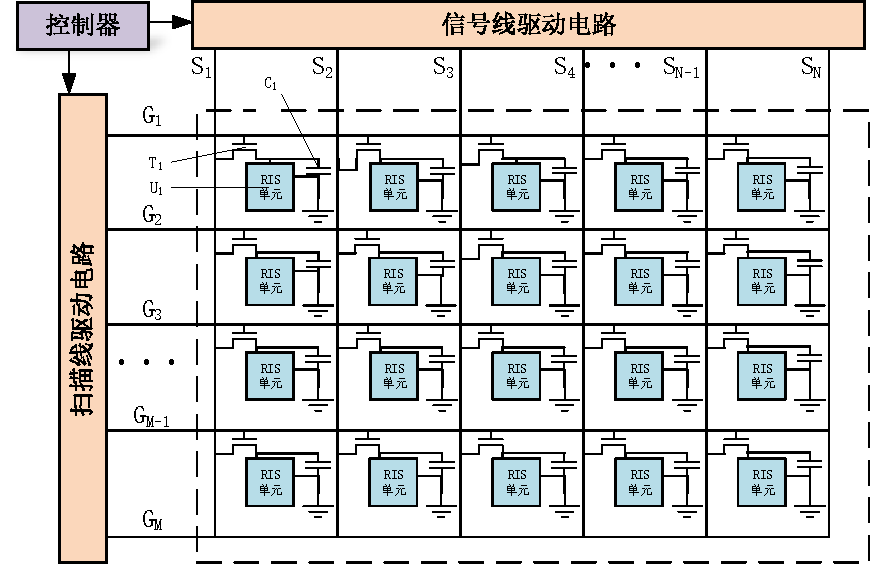
\includegraphics[width=0.8\linewidth]{Figures/MOS.pdf}
\end{generalfig}
如\autoref{fig:MOS}所示为本文设计的基于行列扫描的智能超表面控制方法示意图,图中控制器负责运行智能超表面的控制算法,将运算得到的反射系数矩阵输出给扫描线驱动电路和信号线驱动电路。
剖析左上角的第一个RIS单元及其控制电路:
$U_1$为设计的RIS单元,与它并联的是一个保持电容$C_1$。
单元$U_1$由晶体管$T_1$来控制加载的电压。
当单元$U_1$的行扫描信号脉冲结束后,保持电容$C_1$仍能保持单元$U_1$两端的电压,从而为RIS单元提供持续的驱动电压,直到下一次选通到来。

具体来说,按照本文中的设计,对$M$行$N$列的智能超表面阵列进行$Q ~ \mathrm{bit}$的控制$(Q \ge 1)$时,控制器向扫描线驱动电路发送扫描信号,由扫描线驱动电路选通某一行RIS单元(图中$G_1,G_2,G_3,\cdots,G_{M-1},G_M$)。
接着,控制器向信号线驱动电路发送此行RIS的控制信号,信号线驱动电路在$S_1,S_2,S_3,\cdots,S_{N-1},S_N$上加载$Q ~ \mathrm{bit}$的模拟信号作为控制电压。
此时,被选中行的MOS管导通,电压加载到RIS单元上。
未选通的行的MOS管关断,控制电压由RIS单元对应的保持电容保持。
需要注意的是,控制器需要对RIS面板定时刷新,使保持电容的电压维持在较为稳定的水平。

\begin{generalfig}[htb]{基于行列扫描的智能超表面的某个单元}{fig:MOS-single}
	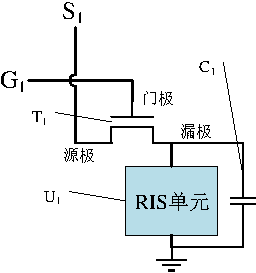
\includegraphics[width=0.4\linewidth]{Figures/MOS-single.pdf}
\end{generalfig}

\autoref{fig:MOS-single}为基于行列扫描的智能超表面的左上角单元示意图,接下来考虑保持电容容值$C_1$的设计。
仍然设RIS面板的尺寸为$M$行$N$列,对RIS面板进行刷新时,每秒更新$f$次,则每次的更新时间为$T=1/f$,即:每帧(Frame)更新时间为$T$,每行更新时间为$T_h=T/M$。
每次刷新时电容的充电时间$dt_{charge}=T_h$,而电容需要保持的时间为$dt_{hold}=T-T_h$。
设RIS单元的阻值为$R_\mathrm{RIS}$,MOS管$T_1$关断时的RIS单元的电流和MOS漏电流之和为$I_{leak}$,关断时允许的电压降为$dV_{hold}$,正常工作时RIS单元的电压为$V_{hold}$。
需要充电的电压$dV_{charge}$为信号线电压与RIS单元电压的电压差,即为晶体管的$V_{ds}$,有:
\begin{equation}
	dV_{charge} = V_{ds}
	\label{eq:V_charge}
\end{equation}
导通充电时,假设充电电流为$I_{charge}$,分析电容充电电荷,有:
\begin{equation}
	I_{charge} \cdot t_{charge}>C_1 \cdot dV_{charge}
	\label{eq:I_charge}
\end{equation}
为保证控制效果,使保持电容的电压维持在较为稳定的水平,要求:
\begin{equation}
	dV_{hold} \le 0.05 \cdot V_{hold}
	\label{eq:V_hold}
\end{equation}
即电压变化率不超过5\%。
关断保持时,对电荷变化建立不等式:
\begin{equation}
	I_{leak} \cdot t_{hold} < C_1 \cdot dV_{hold}
	\label{eq:I_leak}
\end{equation}
其中$I_{leak} = \frac{V_{hold}}{R_\mathrm{RIS}}$。
联立\autoref{eq:V_charge},\autoref{eq:I_charge},\autoref{eq:V_hold}和\autoref{eq:I_leak},可以得到$C_1$的取值范围为:
\begin{equation}
	\frac{20(M-1)}{M} \cdot \frac{T}{R_\mathrm{RIS}} < C_1 < \frac{MI_{charge}T}{V_{ds}}
	\label{eq:C1_value}
\end{equation}

然而对于驱动PIN二极管使能的超表面单元来说,\autoref{eq:C1_value}可能是无解的,这是因为包含PIN二极管的单元的导通电阻$R_\mathrm{RIS}$太小,这时候需要对\autoref{fig:MOS-single}中的电路结构进行改进。
\autoref{fig:Amp}所示为第1行第1列一个RIS单元及采样保持装置的改进结构。
其中场效应管$T_1$的栅极接扫描线$G_1$,源极接信号线$S_1$,漏极接保持电容$C_1$,并连接到运算放大器$A_1$的同向输入端,运算放大器处于单位跟随状态,输出接RIS单元,同时接反向输入端。

\begin{generalfig}[htb]{基于行列扫描的智能超表面的某个单元}{fig:Amp}
	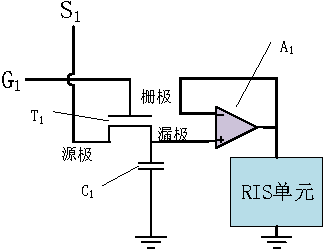
\includegraphics[width=0.5\linewidth]{Figures/Amp.pdf}
\end{generalfig}

选通时间内,场效应管处于导通状态,信号线上的电压被加载到运算放大器的同向输入端并给电容充电;电压经过运算放大器跟随后加载到RIS单元上。
关断时间内,场效应管处于关断状态,由于运算放大器的输入电阻很大,用这种方法可以保持更长时间,且不受RIS单元阻抗的影响。
这种改进电路降低刷新频率,提高稳定性,并且由于运算放大器的输出驱动能力较强,这种电路结构可以驱动阻抗小的RIS单元。

\subsubsection{移位寄存器控制方法}



\subsubsection{智能超表面控制电路}

\subsection{驱动、固件设计}


\subsection{码本设计}


\subsection{本章小结}

本章

\section{总结与展望}\label{sec:conclusion}

\subsection{论文研究工作总结}


\subsection{未来工作展望}

未来,
这是一个参考文献引用的范例\cite{5502350, liang2019large}


\section{公式这么用}

\begin{equation}
	\bm{A}=\begin{bmatrix}
		1  & 2  & 3  & 4  \\
		11 & 22 & 33 & 44 \\
	\end{bmatrix}
	\times\begin{bmatrix}
		22 & 24 \\
		32 & 34 \\
		42 & 44 \\
		52 & 54 \\
	\end{bmatrix}
\end{equation}
或者多个带编号的公式
\begin{eqnarray}
	f_1(x)=12x^2+36x+\sin x\\
	f_2(x)=\sqrt{3}{x^3+3x}
\end{eqnarray}
以上

\section{用图和表的示例}
\subsection{图的使用}
\XeLaTeX 环境下可以使用EPS、PDF、PNG、JPEG、BMP格式的图片,当然也可以用绘图包直接在\LaTeX 中绘制图形,推荐使用宏包tikz。图的环境是figure,但figure环境使用复杂且不自带标题,因此本模板定义了一个通用版本的generalfig,该环境会将figure内的图片居中并设置标签与引用名,同时会让图片位置设置为所有可行位置(htbp,即此处、页顶、页底、独立一页),此选项可以作为可选参数设置。

其使用方法如下:\autoref{fig:50mcopper}


\autoref{fig:50mtest}

\ref{fig:50mcopper}

\ref{fig:50mtest}

\begin{figure}[t!]
	\centering
	\subfloat[df哈哈]{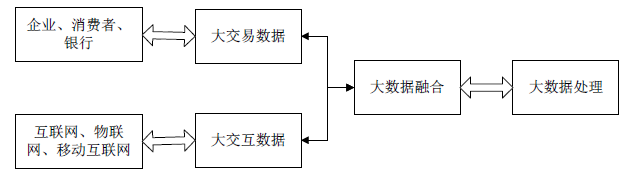
\includegraphics[width=0.5\linewidth]{Figures/data.png}%
		\label{fig:50mphoto}}
	\hfil
	\subfloat[dd]{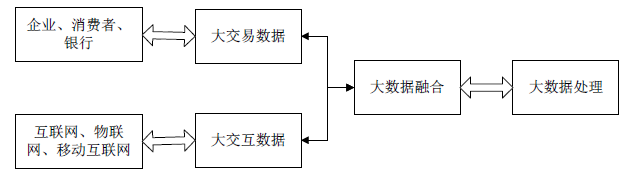
\includegraphics[width=0.5\linewidth]{Figures/data.png}%
		\label{fig:copper}}
	\hfil
	\subfloat[fs]{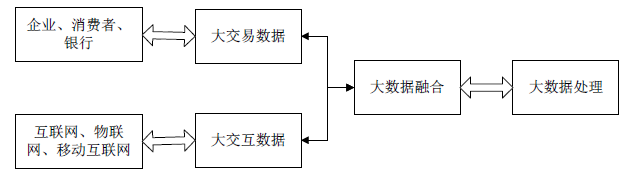
\includegraphics[width=0.5\linewidth]{Figures/data.png}%
		\label{fig:50mgreedy}}
	\hfil
	\subfloat[dfdf]{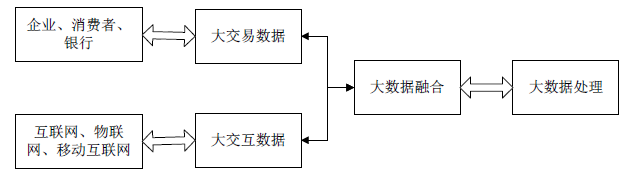
\includegraphics[width=0.5\linewidth]{Figures/data.png}%
		\label{fig:50mcopper}}
	\caption{The 50 m outdoor over-the-air test: (a) the scene of the transmitter and receiver; (b) a copper plate of the same size as the RIS; (c) spectrum when using the RIS; (d) spectrum when using the copper plate.}
	\label{fig:50mtest}
\end{figure}

\begin{figure}[htb]
	\centering
	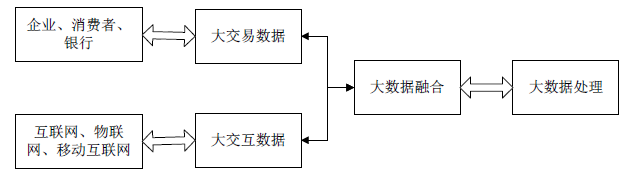
\includegraphics[width=0.5\linewidth]{Figures/data.png}
	\caption{Indoor non-LoS test.}
	\label{fig:through_wall}
\end{figure}

\begin{generalfig}[htb]{大数据信息处理框架}{fig:data}
	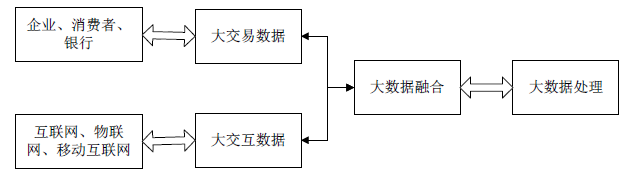
\includegraphics[width=0.4\linewidth]{Figures/data.png}
\end{generalfig}

同时也可以引用该图片例如:\autoref{fig:data}或者图~\ref{fig:data}、。请注意generalfig第一个参数是标题,第二个参数是引用。

\newpage



\begin{thankpage}
	
	\begin{center}
		{\itshape “满纸荒唐言,一把辛酸泪。”}
	\end{center}
	
	\LaTeX

	%{\itshape “流光容易把人抛,红了樱桃,绿了芭蕉。”}
	%{\itshape “文章本天成,妙手偶得之。”}

	%{\itshape “朝发鸡鸣未响,归路晚风凉。汗洒澄池桃李,几度银杏黄。”}

	\begin{figure}[htb]
		\flushright
		
\includegraphics[width=15mm]{Figures/Seal-pxl.pdf}
	\end{figure}

	\begin{flushright}
		2021年5月10日

		于华中科技大学韵苑
	\end{flushright}
	
\end{thankpage}

%生成参考文献
%使用方法:\bibliography{参考文件1文件名, 参考文献2文件名, ...}
\bibliography{Bibs/references_Gradu}

\begin{appendices}
	\section{系统电路原理图}
\end{appendices}

\end{document}




